\section{Experimental setup}
\label{Exp}

In this section, we first describe the dataset used for our experiments and the corresponding classification task. We then delineate the networks used for each of these datasets and the procedure to determine the values of hyperparameters. This is followed by a description of the evaluation metric of the speedup. All the algorithms were implemented in C++. The reported results were obtained on a Ubuntu 14.04.4 LTS system with 32 cores, 128 GB RAM and a clock speed of 2.6 GHz. The GPU used was Nvidia Tesla K40C.

\subsection{Dataset description}
\label{sub:data_desc}

We test the speedups achieved by the parallel implementation on the benchmark dataset: MNIST \cite{mnist_Lecun}. It has been widely used by the machine learning community to compare different learning algorithms. 

MNIST is an image database of handwritten digits, commonly used for training various image processing systems (Figure \ref{fig:mnist}). The task is to classify the digit ($0-9$) in the image. This dataset was derived from NIST's datasets and was formed by mixing the samples from NIST. This mixing was done because the training and testing datasets in the original NIST dataset were obtained from two different groups of people (Census Bureau employees and high school students). The dataset consists of 60,000 training images and 10,000 testing images, each of size $28\times 28$. In our experiments, we further divided the training set into training and validation in 5:1 ratio in order to determine suitable values for the hyperparameters.

\begin{figure}
	\centering
    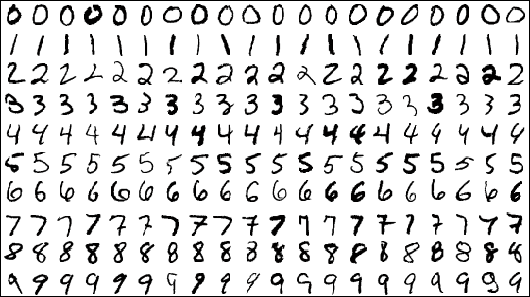
\includegraphics[scale=0.43]{mnist.png}
  	\caption{MNIST dataset}
    \label{fig:mnist}
\end{figure}

\subsection{Network details}
\label{sub:net_det}

We used two different configurations of neural networks:
\begin{itemize}
\item \textbf{Net-1h}: 3 layered network - input (784), one hidden layer (1024) and output layer (10).
\item \textbf{Net-2h}: 4 layered network - input (784), two hidden layers (1024 each) and output layer (10).
\end{itemize}
Both networks had linear activations for input layer and sigmoid activations for all subsequent layers.
The dense layer for each network was initialized using glorot uniform distribution \cite{Glorot2010} and the biases were initialized with zeros.

\subsection{Hyperparameter selection}
\label{sub:hyper_sel}

Hyperparameter selection (model selection) is an important problem in machine learning which involves choosing optimal values for hyperparameters that generalize well on test data.

We chose our learning rate hyperparameter by doing a grid search on the grid $[0.001, 0.002, 0.01, 0.1, 0.5, 1.0]$. As mentioned above, we divide the training set into training and validation (5:1 split). We use different learning rates defined in the grid for learning and test the accuracy on validation data. The rate which gives the highest accuracy on validation is chosen and used to evaluate the performance of the algorithm on test data.

\subsection{Experiments}
\label{sub:exp}
In this paper, we implement different versions of gradient descent algorithm for training neural networks. Some of them used our self-written (slow) linear algebra library (called LINALGLIB henceforth), and others used BLAS. All parallel multicore implementations used 32 execution threads. Keras \cite{Chollet2016} and Theano \cite{Theano2012, Bergstra2010} based implementations also use BLAS. The implementations are as follows:
\begin{itemize}
\vspace{-8pt}
\item Naive Serial, Multicore Parallel, GPU Parallel
\vspace{-4pt}
\item Fast Serial, Fast Parallel
\vspace{-4pt}
\item Theano Serial, Theano Parallel, Theano GPU
\vspace{-8pt}
\end{itemize}
Detailed description of implementations is given in table \ref{tab:exp}.

\begin{table}[h]
\centering
\begin{tabular}{|c|c|c|c|}
\hline
\textbf{Name} & \textbf{Parallelism} & \textbf{Lin. Algebra} & \textbf{Platform} \\
 & & \textbf{Library} & \\
\hline
Naive & - & LINALGLIB & C++ \\
Serial & & & \\
\hline
Multicore & Training & LINALGLIB & Pthreads, \\
Parallel & examples & & C++ \\
\hline
GPU & Training & LINALGLIB & CUDA, \\
Parallel & examples & & C++ \\
\hline
Fast & - & BLAS & C++ \\
Serial & & & \\
\hline
Fast & Matrix & BLAS & C++ \\
Parallel & operations & & \\
\hline
Theano & - & BLAS & Keras, \\
Serial & & & Theano \\
\hline
Theano & Training ex., & BLAS & Keras, \\
Parallel & Matrix ops & & Theano\\
\hline
Theano & Training ex., & BLAS & Keras, \\
GPU & Matrix ops & & Theano \\
\hline
\end{tabular}
\caption{Detailed description of implementations}
\label{tab:exp}
\end{table}

\subsection{Evaluation methodology}
\label{sub:eval}

To evaluate our approach and quantify the usefulness of parallelization, we use speedup as our primary measure.
We compute speedup for each parallel implementation with respect to its serial counterpart on the same network configuration.
For each parallel implementation we also compute the running time per training epoch (in seconds) and the amount of computation per epoch (in gigaflops) since speedup alone may sometimes be misleading and does not capture the efficiency of parallel implementation. These measures are independent of serial implementation and can be used to supplement the speedup metric.